\documentclass[11pt]{article}
\usepackage{amsmath,amsthm,amsfonts,amssymb,amscd}
\usepackage{cancel}
\usepackage[shortlabels]{enumitem}
\usepackage{fancyhdr} 
\usepackage{fullpage}
\usepackage[top=2cm, bottom=4.5cm, left=2.5cm, right=2.5cm]{geometry}
\usepackage{graphicx}
\usepackage{hyperref}
\usepackage{listings} %for code
\usepackage{mathtools}
\usepackage{multicol}
\usepackage{pgfplots}
\usepackage{tabularx}
\usepackage{tikz-cd,tikz}
\usepackage{todonotes}
    \pgfplotsset{
        compat=1.12,
    }
\usepackage[breakable,skins,most]{tcolorbox}
\usepackage{verbatim}
\usepackage{xcolor}
\usepackage{ytableau}

\newtcolorbox{greybox}[1]{%untitled
colback=gray!5!white,
colframe=gray!75!black,
fonttitle=\bfseries,
title=#1}

\newtcolorbox{defbox}[1]{%untitled
colback=blue!5,
colframe=blue!50,
fonttitle=\bfseries,
title=#1}

\newtcolorbox{exbox}[1]{
colback=green!5,
colframe=green!75!black,
fonttitle=\bfseries,
title=Example {(#1)}}

\newtcolorbox{pbox}[1]{
colback=violet!5,
colframe=violet!50,
fonttitle=\bfseries,
title=Proposition #1}

\newtcolorbox{quesbox}{
colback=magenta!5,
colframe=magenta!50,
fonttitle=\bfseries,
title=??}

\newtcolorbox{qbox}{
colback=red!5,
colframe=red!75,
fonttitle=\bfseries,
title=Question}

\newtcolorbox{thbox}[1]{
colback=violet!5,
colframe=violet!75,
fonttitle=\bfseries,
title=Theorem (#1)}

\hypersetup{%
  colorlinks=true,
  linkcolor=blue,
  linkbordercolor={0 0 1}
}
 
\setlength{\parindent}{0.0in}
\setlength{\parskip}{0.05in}

% Edit these as appropriate
\newcommand\course{UCI 2024}             
\newcommand\Name{Max LaFortune}

% Macros
\newcommand{\A}{\mathbb{A}}
\newcommand{\C}{\mathbb{C}}
\newcommand{\F}{\mathbb{F}}
\newcommand{\calH}{\mathcal{H}}
\newcommand{\calM}{\mathcal{M}}
\newcommand{\N}{\mathbb{N}}
\newcommand{\calP}{\mathcal{P}}
\newcommand{\Q}{\mathbb{Q}}
\newcommand{\R}{\mathbb{R}}
\newcommand{\Z}{\mathbb{Z}}

\newcommand{\all}{\ \forall \ }
\newcommand{\ans}{\textbf{A: \ }}
\newcommand{\aut}{\text{Aut}}
\newcommand{\blue}[1]{\textcolor{blue}{#1}}
\newcommand{\bs}{\backslash}
\newcommand{\cross}{\times}
\newcommand{\Def}[2]{\begin{defbox}{#1}{#2}
\end{defbox}}
\newcommand{\defn}{\textbf{\underline{Definition}}}
\newcommand{\ex}[2]{\begin{exbox}{#1}{#2}
\end{exbox}}
\newcommand{\exist}{ \ \exists \ }
\newcommand{\ext}{\text{Ext}}
\newcommand{\facts}{\textbf{\underline{Facts}}}
\newcommand{\green}[1]{\textcolor{green}{#1}}
\newcommand{\Hom}{\text{Hom}}
\newcommand{\id}[1]{\begin{quesbox}{#1}
\end{quesbox}}
\newcommand{\iso}{\cong}
\newcommand{\kw}[1]{\textit{#1}}
\newcommand{\la}{\lambda}
\newcommand{\prop}[2]{\begin{pbox}{#1}{#2}
\end{pbox}}
\newcommand{\Ques}[1]{\begin{qbox}{#1}
\end{qbox}}
\newcommand{\red}[1]{\textcolor{red}{#1}}
\newcommand{\sect}[1]{\section*{#1}}
\newcommand{\ssect}[1]{\subsection*{#1}}
\newcommand{\thm}[2]{\begin{thbox}{#1}{#2}
\end{thbox}}

\title{}
\pagestyle{fancyplain}
\headheight 35pt
\lhead{\Name}
\chead{\textbf{\Large Numerical Semigroups}}
\rhead{\course}
\lfoot{}
\cfoot{}
\rfoot{\small\thepage}
\headsep 1.5em

\setcounter{tocdepth}{3}
\setcounter{secnumdepth}{3}

\begin{document} 
\tableofcontents

\newpage
\section*{Notation}
\addcontentsline{toc}{section}{Notation}
This table was created by Kaylee. 

\begin{table}[!h]
    \centering
    \begin{tabularx}{\textwidth}{c|X}
        Notation & Item \\
        \hline \\
        $\lambda_i$ & $i$-th part of partition $\lambda$ \\
        $|\lambda|$ & size of $\lambda$, i.e. $\sum_{i=0}^t\lambda_i$ \\
        $p(n)$ & partition counting function by size, $p(n) =  \#\{\text{partitions of }n\}$\\
         $\mathcal{H}(\lambda)$ & multiset of hook lengths \\
         $H(\lambda)$ & set of hook lengths \\
         $\lambda ', \tilde{\lambda}$ & conjugate of a partition $\lambda$ \\
         $g(S)$ & genus of $S$, i.e. number of gaps of $S$ \\
         $F(S)$ & Frobenius number of $S$ \\
         $PF(S)$ & set of pseudo-Frobenius numbers of $S$ \\
         $t(S)$ & the type of $S$, that is, $|PF(S)|$ \\
         $\langle n_1,..., n_k \rangle$ & numerical semigroup generated by $\{n_1, ...,n_k\}$ \\
         $m(S)$ & multiplicity of $S$, i.e. the smallest minimal generator of $S$ \\
         $e(S)$ & the embedding dimension of $S$, i.e. the number of minimal generators of $S$ \\
         $\lambda(S)$ & the partition built from the numerical semigroup $S$, \newline i.e. the enumeration of $S$ \\
         $P(S)$ & partition/numerical set counting function by associated numerical semigroup \\
         $T^*$& the dual of numerical set $T$ \\
         $\mathcal{M}(S)$& the void of $S$ \\
         $(\mathcal{M}(S), \preceq)$& the void poset of $S$ \\
         $Ap(S;n)$ & $= \{ x \in S | x - n \not \in S \}$ The Apery set. \\
         & \\
         & \\
    \end{tabularx}
\end{table}


\newpage 
\section*{Week 1}
\addcontentsline{toc}{section}{Week 1}
\Def{Definition}{ The \textbf{type} of $S$ is $|PF(S)| = t(S)$. 

In words, the type is the number of pseudofrobenius numbers.

Note: $t(S) \leq 2g(S) - F(S)$}


\Def{Definition}{

A numerical semigroup $S$ for which $x \in S \iff F(S) - x \not \in S$ is   \textbf{symmetric}. 

A numerical semigroup $S$ is \textbf{pseudo-symmetric} if $F(S)$ is even and $M(S) = \{ \frac{1}{2} F(S) \}.$

If $t(S) = 2g(S) - F(S) $ then $S$ is \textbf{almost symmetric}. 

Note: symmetric $\implies$ almost symmetric.}

Symmetry, type and partitions are closely related:

$M(S) = \emptyset \iff P(S) =1 \iff S$ is symmetric $\iff t(S) = 1 $ 

$|M(S)| = 1 \iff $ $S$ is pseudo-symmetric $ \implies t(S) = 2 \implies P(S) = 2$

$t(S) = 3 \implies P(S) \in \{ 2, 3, 4 \}$

\newpage
\section*{Week 2}
\addcontentsline{toc}{section}{Week 2}

\subsection*{July 3rd \& 4th}
\addcontentsline{toc}{subsection}{July 3rd \& 4th} 
I am going to look at void posets as that is something I have not spent very much time on. Here is some necessary background:

\Def{Definition}{The \textbf{void} of $S$, denoted $\mathcal{M}(S)$ is the union of all the sets $\{x, F(S) -x\}$ for all $x$ where both $x$ and $F(S)-x$ are gaps. Note $\mathcal{M}(S) \subseteq \N \setminus S$.

The \textbf{void poset} of $S$, denoted $(\mathcal{M}(S), \preceq)$, is the void, $\mathcal{M}$ equipped with the partial ordering $\preceq$, where
    $$x \preceq y \text{ if } y-x \in S \text{ for all } x, y \in \mathcal{M}(S).$$
}

\Def{Definition}{$x \in \mathcal{M}(S)$ is \textbf{maximal} if $x \preceq y \implies x = y$.

$x$ is a \textbf{pseudofrobenius number} if $x \not\in S$ and $x+s \in S$ for any $s \in S \backslash  \{ 0\}$. We denote the set of pseudofrobenius numbers by $PF(S)$.}

\prop{}{ The maximal elements of $(\calM(S),\preceq)$ are the elements of $PF(S) \backslash F(S)$.}

\Def{Definition}{Let $I \subseteq M(S).$ }

Now that I have gathered all this information in one place I am going to write/find code that displays the void poset of a given numerical semigroup (with the edges labeled by difference?). This should be useful because it will allow me to easily visualize many posets and so recognize patterns faster. 

Deepesh sent code, the first in the discord code channel that has to do with this. 







\newpage 
\section*{Week 3}
\addcontentsline{toc}{section}{Week 3}

\subsection*{July 11th}
\addcontentsline{toc}{subsection}{July 11th} 
I wrote code that takes all numerical semigroups of a certain genus, prints its generators and the number of edges in it's gap poset to a csv file so it can be easily added to a spreadsheet.

\begin{lstlisting}[language=python]
    def GapPoset(S): #print gap poset        #Modified from VoidPoset which was taken from Deepesh
        GG = S.Gaps()
        L = []
        for i in GG:
            for j in GG:
                if j-i in S:
                    L.append([i,j])
        GP = Poset([GG,L])
        # show(GP)
        return GP

    def GapPosetEdges(S): #prints number of edges in GapPoset 
        GP = GapPoset(S)
        A = GP.cover_relations()
        B = len(A)
        return B

    genus = 
    sgps = NumericalSemigroup.SemigroupsWithGenus(genus)

    L = []
    M = []
    for S in sgps: 
        GE = S.gens
        type(GE)
        a = GapPosetEdges(S)
        b = str(a)
        L.append(GE)
        M.append(b)
    length = len(L)
    with open('/home/samwisega/genusedges.csv', 'w') as file:
        for i in range(length):
            file.write('"')
            file.write(str(L[i]))
            file.write('",')
            file.write(M[i])
            file.write('\n')
\end{lstlisting}

\subsection*{July 13th}
\addcontentsline{toc}{subsection}{July 13th} 
\subsubsection*{What should I do?}

Friday I asked Professor Kaplan what I should work on. Here is some background he provided: 

\# effective gens of S $= eg(S)$
\thm{O'Dorney}{$$\lim_{g \to \infty} \frac{\# \{S | g(S) = g, eg(S) = h \}}{N(g)} = \frac{1}{\varphi^{n+2}}$$}

\Ques{Fix $m$. What is $$\lim_{g \to \infty} \frac{\# \{S | g(S) = g, m(S)=m, eg(S) = h \}}{\# \{ S | g(S) = g, m(S) = m\}} ?$$}

Claim: $\# \{ S | g(S) = g, m(S) = 3, eg(S) = 0\} \leq \# \{ S | g(S) = g, m(S) = 3, eg(S) \geq 2\}$

\subsubsection*{Code}
I wrote code that does a breadth first traversal of the numerical semigroup tree looking at all semigroups of multiplicity m, up to genus g and counts their children. 

\begin{lstlisting}[language=python]
gap.eval('LoadPackage("numericalsgps")')
load('/home/samwisega/Downloads/NumericalSemigroup.sage')

def Children(S): #print children of S    #Max & Deepesh
    GENS = S.gens 
    F = S.FrobeniusNumber() 
    MULT = GENS[0]
    L = []
    for i in GENS: 
        if F < i: 
            NEWGENS = []
            for x in GENS: 
                if x != i: 
                    NEWGENS.append(x)
            NEWGENS.append(i + MULT)
            NEWGENS.append(i + MULT + 1)
            L.append(NumericalSemigroup(NEWGENS))
    return L   

def Genus(S): 
    return len(S.Gaps())

class Node:
    def __init__(self, value):
        self.value = value
        self.children = []
        
    def add_child(self, child_node):
        self.children.append(child_node)
        
class Tree:
    def __init__(self, root_value):
        self.root = Node(root_value)

    def find(self, value, node=None):
        if node is None:
            node = self.root
        if node.value == value:
            return node
        for child in node.children:
            result = self.find(value, child)
            if result is not None:
                return result
        return None

    def insert(self, parent_value, child_value):
        parent_node = self.find(parent_value)
        if parent_node is None:
            raise ValueError(f'Parent node with value {parent_value} not found.')
        child_node = Node(child_value)
        parent_node.add_child(child_node)    

    def display(self, node=None, level=0):
        if node is None:
            node = self.root
        print(' ' * level * 2 + str(node.value))
        for child in node.children:
            self.display(child, level + 1)

from collections import deque 
from collections import Counter

def branchmult(MAXG, m, S): #prints elements with multiplicity m in the num sgp tree starting at S
    GENS = S.gens
    tree = Tree(GENS)
    visited = []
    queue = deque([tree.root])
    g = Genus(S)
    numClst = []
    
    with open('/home/samwisega/MultChild.csv', 'w') as file:
        file.write('Genus,Generators,Number of Children\n')
        
        while queue and g <= MAXG:
            node = queue.popleft()
            f = Genus(NumericalSemigroup(node.value))
            visited.append(node.value)
            current_gen = NumericalSemigroup(node.value)
            C = Children(current_gen)
            numC = len(C)
            numClst.append(numC)
            
            # Print the genus, current semigroup and number of children  
            # to a csv file 
            file.write(str(g))
            file.write(',"')
            file.write(str(node.value))
            file.write('",')
            file.write(str(numC))
            file.write('\n')

            for c in C:  
                tree.insert(node.value, c.gens)  
                # Insert the new semigroup into the tree
                if m in c.gens:
                    queue.append(Node(c.gens))  
                    # Append the new node to the queue
            
            nextnode = queue[0]
            g = Genus(NumericalSemigroup(nextnode.value))
            
            if f < g: 
                print('genus', f, Counter(numClst))
                numClst = []
\end{lstlisting}

\subsubsection*{Results}
First I ran this:
\begin{lstlisting}[language=python]
    S = NumericalSemigroup([3, 4, 5])
    branchmult(150,3,S)
\end{lstlisting}
but I'm impatient and a pattern was already becoming clear so I stopped it at genus = 136. 

I have uploaded the csv file to a google sheet titled \href{https://docs.google.com/spreadsheets/d/1xaydWKcqVwpPp5F2e6hJjlvRE8n7Usz3lbObVt-hW9E/edit?usp=sharing}{MultChild}, I made an error in formatting the semigroup gaps so it is easier to view m=3, g=100. 

This also printed the number of times a semigroup has n children per genus for multiplicity 3. I also have pasted it into \href{https://docs.google.com/document/d/1cEPls2GodRP2_9fGsHNTLlVaDbv5GTP3PEub-oqsaGY/edit?usp=sharing}{this google doc} but to make viewing easier, here it is up to genus 32. 

genus 2   Counter({3: 1}) \\
genus 3   Counter({2: 1, 0: 1}) \\
genus 4   Counter({2: 1, 0: 1})\\
genus 5   Counter({2: 1, 1: 1})\\
genus 6   Counter({2: 1, 1: 1, 0: 1})\\
genus 7   Counter({2: 1, 1: 1, 0: 1})\\
genus 8   Counter({1: 2, 2: 1})\\
genus 9   Counter({1: 2, 2: 1, 0: 1})\\
genus 10   Counter({1: 2, 2: 1, 0: 1})\\
genus 11   Counter({1: 3, 2: 1})\\
genus 12   Counter({1: 3, 2: 1, 0: 1})\\
genus 13   Counter({1: 3, 2: 1, 0: 1})\\
genus 14   Counter({1: 4, 2: 1})\\
genus 15   Counter({1: 4, 2: 1, 0: 1})\\
genus 16   Counter({1: 4, 2: 1, 0: 1})\\
genus 17   Counter({1: 5, 2: 1})\\
genus 18   Counter({1: 5, 2: 1, 0: 1})\\
genus 19   Counter({1: 5, 2: 1, 0: 1})\\
genus 20   Counter({1: 6, 2: 1})\\
genus 21   Counter({1: 6, 2: 1, 0: 1})\\
genus 22   Counter({1: 6, 2: 1, 0: 1})\\
genus 23   Counter({1: 7, 2: 1})\\
genus 24   Counter({1: 7, 2: 1, 0: 1})\\
genus 25   Counter({1: 7, 2: 1, 0: 1})\\
genus 26   Counter({1: 8, 2: 1})\\
genus 27   Counter({1: 8, 2: 1, 0: 1})\\
genus 28   Counter({1: 8, 2: 1, 0: 1})\\
genus 29   Counter({1: 9, 2: 1})\\
genus 30   Counter({1: 9, 2: 1, 0: 1})\\
genus 31   Counter({1: 9, 2: 1, 0: 1})\\
genus 32   Counter({1: 10, 2: 1})\\

Notice a pattern? Yea, opening the google doc is a waste of time, it shows exactly what you would expect. 
\newpage
\begin{itemize}
    \item for $m = 3, g > 2, \# \{S | eg(S) = 0\} \leq \# \{S | eg(S) = 2\}$  
    \item when $g$ is odd the only semigroup with 2 effective generators is generated by \\
    $\langle 3, 3(g+1)/2 - 1, 3(g+1)/2 +1  \rangle$, when $g$ is even it is generated by $\langle 3, 3g/2 + 1, 3g/2+2 \rangle $. 
    
    \item when $g = 0$ or $1 \mod 3$, the semigroup generated by $\langle 3, g+1 \rangle$ has 0 effective generators. When $g = 2 \mod 3$ there is no semigroup with 0 effective generators.
    
    \item In genus $g$ there are $\lfloor (g+1)/3\rfloor -1$ semigroups with $1$ effective generator. 
\end{itemize}

Therefore for semigroups with multiplicity $m=3$ and $h > 0$ we have 
$$\lim_{g \to \infty} \frac{\# \{S | g(S) = g, eg(S) = h \}}{\# \{ S | g(S) = g\}} = 1$$

\section*{Week 4}
\addcontentsline{toc}{section}{Week 4}

\subsection*{July 15th}
\addcontentsline{toc}{subsection}{July 15th} 
Today I am working on formalizing what I saw on the 13th. 

Consider the Kunz coordinates associated to a numerical semigroup with multiplicity $m=3$. For $Ap(S) = \{ 3, 3k_1+1, 3k_2+2\}$ we have the associated coordinates $(k_1, k_2).$

If $S \to (k_1, k_2)$ then the children of $S$ will be 
\begin{itemize}
    \item $(k_1 + 1, k_2)$ when $k_2 + 1 \leq k_1 < 2k_2 + 1$,
    \item $(k_1, k_2 + 1)$ when $k_1 \leq k_2 < 2k_1$.
\end{itemize}
Note: If $k_1=k_2$ or $k_1 = k_2 + 1$ both $(k_1 + 1, k_2)$ and $(k_1, k_2 + 1)$ will be children. If $k_1 = 2k+1$ or $k_2 = 2k_1$ there will be no children.

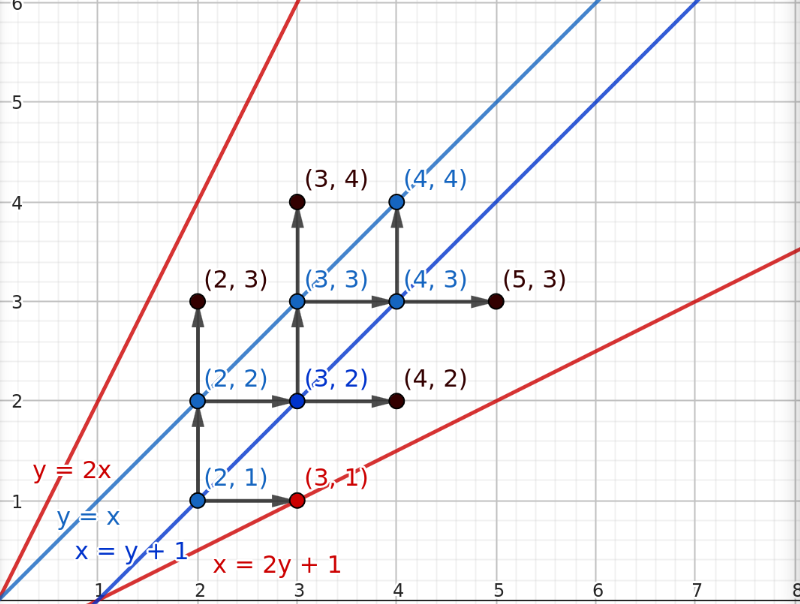
\includegraphics[scale=0.3]{Max/images/Screenshot from 2024-07-15 13-01-52.png}

\subsection*{July 17th}
\addcontentsline{toc}{subsection}{July 17th} 
[source 1] https://cdoneill.sdsu.edu/whatis/kunz.html

[source 2] Numerical semigroups, polyhedra, and posets I: the group cone. Nathan Kaplan and Christopher O'Neil. 

Let $N_m(g)$ denote the number of numerical semigroups $S$ with $m(S) = m$ and $g(S) = g.$

For $m \geq 3$ there is a Kunz polyhedron $P_m \subseteq \R^{m-1}$. Each integer point in $P_m$ corresponds to a numerical semigroup $S$ with multiplicity $m$. 

The bounding inequalities for the Kunz polyhdrom $P_m \subseteq \R^{m-1}$ are 
$$x_i + x_j \geq x_{i+j} \ \text{for} \ 1 \leq i \leq j \leq m - 1 \ \text{with} \ i + j < m$$
$$x_i + x_j + 1 \geq x_{i+j-m} \ \text{for} \ 1 \leq i \leq j \leq m - 1 \ \text{with} \ i + j > m$$

\end{document}